\documentclass{article}

\usepackage[utf8]{inputenc}
\usepackage{microtype}
\usepackage{graphicx}
\usepackage{amsmath,amssymb}
\usepackage{hyperref}
\usepackage{tikz}
\usepackage{enumitem}
\usepackage{caption}
\usepackage{subcaption}
\usepackage{url}

\usetikzlibrary{positioning,fit,arrows.meta,calc}

\let\originalfootnotesize\footnotesize
\let\oldverbatim\verbatim
\let\oldendverbatim\endverbatim
\renewenvironment{verbatim}{\originalfootnotesize\oldverbatim}{\oldendverbatim}

\title{Erlang OS.1: Bytecode Virtualized POSIX Systems Architecture and Engineering}

\author{Magnus Ericsson \texttt{root@5ht.co}}
\date{\today}

\begin{document}
\maketitle

\begin{abstract}
We present the \textbf{Erlang OS.1} systems architecture that reinterprets the traditional POSIX process model through the lens of the Erlang/OTP virtual machine.
Built on a minimal Alpine Linux base, the design elevates the BEAM to the primary unit of isolation, lifecycle management, and privilege separation.
A privileged System BEAM owns all direct kernel interactions, while one or more unprivileged User BEAMs host graphical sessions (including the X11 server), window managers, and application workloads.
All software is delivered as signed OTP releases; native code is minimised and confined.
The architecture retains Linux kernel isolation primitives (cgroups, namespaces, seccomp) as a hard outer boundary while exploiting OTP supervision, hot code loading, and distribution for fine-grained internal control.
We articulate five design rules, detail the resulting software structure, examine device capability transfer,
multi-seat operation, and the placement of the display server, and conclude with an assessment of the model's
applicability to mission-critical defense appliances, aerospace systems, and as a modern, soft real-time replacement for legacy Ada.
\end{abstract}

\newpage
\tableofcontents
\newpage

%----------------------------------------------------------------------
\section{Introduction}
%----------------------------------------------------------------------

Contemporary general-purpose operating systems rely on the POSIX process as the fundamental unit of isolation and resource accounting.
While robust, this model incurs substantial context-switch and inter-process communication costs and offers only coarse supervision semantics.
Concurrently, language runtimes such as the Erlang BEAM have demonstrated that lightweight, memory-safe processes under hierarchical supervision can deliver high reliability for concurrent and distributed workloads.

This paper explores a hybrid architecture in which the BEAM becomes the dominant container for application logic on a POSIX substrate.
We retain a minimal Linux kernel (Alpine Linux with musl libc and a stripped userland) for hardware support and hard isolation, yet organise almost all system and user software as OTP applications executing inside carefully separated BEAM instances.
The resulting system treats verified Erlang releases as the unit of deployment and the BEAM itself as a capability-mediated container.

The design is motivated by three observations:
\begin{enumerate}[nosep]
  \item OTP supervision trees provide richer failure isolation and recovery than traditional init systems;
  \item a single, auditable runtime reduces the attack surface associated with polyglot scripting and ad-hoc native binaries;
  \item modern kernel facilities (cgroups v2, namespaces, seccomp-bpf, file-descriptor passing) can still enforce strong boundaries around each BEAM operating-system process.
\end{enumerate}

We do not claim that the architecture is a drop-in replacement for a general-purpose Linux distribution.
Rather, we argue that it constitutes a coherent substrate for mission-critical defense appliances, aerospace command-and-control (C2) systems, and high-assurance vehicles. In these environments, the benefits of a uniform, supervised, bytecode-verified execution environment offer a compelling, memory-safe alternative to legacy Ada and traditional RTOS deployments, fundamentally outperforming them in runtime resilience, hot-code reloading for zero-downtime patching, and native distributed supervision.

\section{Architecture}

%----------------------------------------------------------------------
\subsection{Design Rules}
%----------------------------------------------------------------------

Five invariants govern the architecture.
They are stated first because every subsequent mechanism is derived from them.

\begin{enumerate}[label=\textbf{R\arabic*}]
  \item \textbf{System BEAM ownership.}
  The System BEAM is the sole entity permitted to perform privileged kernel operations (device open, mount, network configuration, capability grants).
  No User BEAM holds raw access to privileged interfaces.

  \item \textbf{User BEAMs are untrusted.}
  Communication between User BEAMs and the System BEAM occurs exclusively through narrow, explicitly capability-limited channels: Erlang distribution protected by TLS and cookies, or length-prefixed Unix-domain sockets carrying authenticated messages.
  No ambient authority is assumed.

  \item \textbf{OTP releases only.}
  Every loadable component is a signed OTP release.
  Ad-hoc scripts, unstructured binaries, and unsigned code are rejected by the loader.
  Verification precedes execution.

  \item \textbf{Native code minimisation.}
  Ports are preferred to NIFs.
  Any remaining NIFs are small, audited, and confined to a trusted set residing in the System BEAM or in a dedicated privileged helper.
  The User BEAM native surface is reduced to the absolute minimum required for device interaction and the display server.

  \item \textbf{Kernel isolation remains primary.}
  Each BEAM executes inside its own set of Linux namespaces and cgroups.
  The kernel, not the BEAM, provides the hard isolation boundary that the managed language runtime cannot guarantee alone.
\end{enumerate}

These rules deliberately invert the conventional layering: the language runtime becomes the primary organisational principle, while the kernel supplies an outer, coarse-grained enforcement layer.

%----------------------------------------------------------------------
\subsection{System Description}
%----------------------------------------------------------------------

\subsubsection{Base Layer}

The foundation is Alpine Linux configured for minimalism:
\begin{itemize}[nosep]
  \item Linux kernel with necessary drivers and security modules;
  \item musl libc;
  \item busybox (or a further-reduced toolset);
  \item a tiny init (s6, a custom static binary, or a supervised OpenRC instance) whose sole permanent duty is to launch and supervise the System BEAM.
\end{itemize}

The init process is intentionally thin; once the System BEAM is running, nearly all policy resides inside OTP supervision trees.

\subsubsection{System BEAM}

The System BEAM runs with elevated privileges (or with a carefully curated set of Linux capabilities) and owns:
\begin{itemize}[nosep]
  \item network configuration and routing;
  \item storage discovery, mounting, and volume management;
  \item device event aggregation (via netlink, udev, or a minimal eudev replacement);
  \item power management, timekeeping, and logging;
  \item a capability broker that grants file descriptors and limited rights to User BEAMs.
\end{itemize}

It never opens a graphical display connection and never loads untrusted application code.

\subsubsection{User BEAM}

Each User BEAM corresponds to a seat or a logged-in user and is unprivileged.
It contains:
\begin{itemize}[nosep]
  \item the X11 server (rootless Xorg, Xwayland, or a research minimal server);
  \item the window manager (an OTP application communicating with the X server through a C Port);
  \item compositor and status-bar components if required;
  \item all user-facing OTP applications;
  \item a restricted distribution or socket endpoint back to the System BEAM.
\end{itemize}

Multiple User BEAMs may coexist, enabling multi-seat operation or strong separation between concurrent user sessions.

\begin{figure}[ht]
\centering
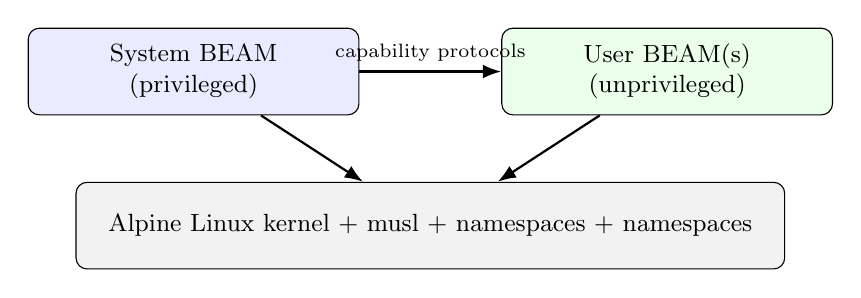
\begin{tikzpicture}[
  box/.style={draw, rounded corners, align=center, minimum height=1.1cm, font=\small},
  sys/.style={box, fill=blue!8, minimum width=4.2cm},
  usr/.style={box, fill=green!8, minimum width=4.2cm},
  arrow/.style={-Latex, thick}
]
\node[sys] (sys) {System BEAM\\(privileged)};
\node[usr, right=1.8cm of sys] (usr) {User BEAM(s)\\(unprivileged)};
\node[box, fill=gray!10, below=1.4cm of $(sys)!0.5!(usr)$, minimum width=9cm] (alpine)
  {Alpine Linux kernel + musl + namespaces + namespaces};
\draw[arrow] (sys) -- node[above,font=\scriptsize]{capability protocols} (usr);
\draw[arrow] (sys) -- (alpine);
\draw[arrow] (usr) -- (alpine);
\end{tikzpicture}
\caption{High-level organisation of the dual-BEAM architecture.}
\label{fig:overview}
\end{figure}

%----------------------------------------------------------------------
\subsection{Critical Architectural Aspects}
%----------------------------------------------------------------------

\subsubsection{Display Server Placement}

Placing the X11 server inside the User BEAM follows directly from Rules~1 and~2.
Graphics are session-scoped; a crash or compromise of the display server must not affect system services.
Modern rootless Xorg and Xwayland already operate without permanent root privileges, aligning with the untrusted nature of the User BEAM.

A long-term research direction is a minimal X server implemented primarily as an Erlang Port or a tightly audited NIF.
Such a server would give the runtime complete control over the protocol surface at the cost of substantial engineering effort; it is therefore regarded as a future option rather than a near-term requirement.

\subsubsection{Device Capability Transfer}

The System BEAM retains ownership of DRM/KMS and input devices.
When a User BEAM is spawned, the System BEAM performs the following sequence:

\begin{enumerate}[nosep]
  \item opens the required device nodes;
  \item applies any necessary ioctls or mode setting that demand privilege;
  \item transmits the resulting file descriptors to the User BEAM via \texttt{SCM\_RIGHTS} over a Unix-domain socket, or via a controlled Erlang distribution payload;
  \item records the grant so that revocation remains possible.
\end{enumerate}

The User BEAM never possesses the ambient authority to open those devices itself.
This pattern realises a classic capability model on top of POSIX file descriptors.

\subsubsection{User BEAM Supervision Tree}

A representative supervision hierarchy inside a User BEAM is:

\begin{verbatim}
user_sup
+-- x11_server_sup          % Port or external OS process wrapper
|   +-- x11_port
+-- wm_sup
|   +-- wm_x11              % C Port talking to local X server
|   +-- wm_event
|   +-- wm_windows
|   +-- wm_workspace
|   +-- wm_layout
|   +-- wm_keybind
+-- session_apps_sup        % user OTP applications
+-- system_bridge           % authenticated channel to System BEAM
\end{verbatim}

The X server and the window manager are siblings under a common supervisor, permitting coordinated restart strategies while preserving isolation from ordinary application failures.

\subsubsection{Multi-Seat and Multi-User BEAM Design}

Each seat is assigned its own User BEAM.
The System BEAM acts as a seat manager:
\begin{itemize}[nosep]
  \item allocates device capabilities per seat;
  \item enforces cgroup and namespace separation;
  \item mediates any cross-seat communication through explicit policy.
\end{itemize}

Because each User BEAM is an ordinary OS process wrapped by kernel isolation primitives, the failure or compromise of one seat does not automatically propagate to another.
Erlang distribution between User BEAMs, if enabled at all, is subject to the same capability discipline as communication with the System BEAM.

%----------------------------------------------------------------------
\subsection{Security Considerations}
%----------------------------------------------------------------------

The security model is layered:

\begin{itemize}
  \item \textbf{Kernel layer} --- namespaces, cgroups v2, seccomp-bpf filters, and capability bounding sets applied to every BEAM process.
  \item \textbf{BEAM layer} --- OTP release signatures, restricted distribution cookies, and the absence of ambient authority inside User BEAMs.
  \item \textbf{Protocol layer} --- all System--User interactions are typed, versioned, and capability-bearing; no ambient file-system or device access is granted.
\end{itemize}

The principal residual risks are:
\begin{enumerate}[nosep]
  \item vulnerabilities inside the BEAM implementation itself;
  \item defects in the small set of trusted NIFs or Ports;
  \item misconfiguration of the capability broker.
\end{enumerate}

These risks are mitigated by minimising native code, by continuous auditing of the trusted computing base, and by the ability to restart individual User BEAMs without system-wide disruption.

Furthermore, this multi-layered security posture directly satisfies stringent defense-in-depth and Zero Trust Architecture (ZTA) requirements mandated in modern defense technologies. By combining Linux kernel namespaces with BEAM bytecode verification, the architecture ensures that a compromised component cannot escalate privileges or pivot within the network.

%----------------------------------------------------------------------
\subsection{Related Work}
%----------------------------------------------------------------------

The architecture sits at the intersection of several lines of research.
Erlang-on-Xen and the LING project demonstrated BEAM-centric systems on top of a hypervisor.
GRiSP and similar embedded platforms run OTP applications close to the hardware.
Unikernel approaches (MirageOS, IncludeOS) eliminate the general-purpose OS entirely.
Container systems (Docker, Podman, Firecracker) provide strong isolation at the cost of heavier runtime footprints.

Our design differs by retaining a full Linux kernel for driver support while elevating the BEAM to the primary organisational and supervisory unit.
It is closer in spirit to a language-based operating system that still exploits POSIX device models, rather than a pure unikernel or a conventional container host.

In the domain of high-integrity systems, legacy Ada and SPARK have long provided compile-time safety guarantees. However, Erlang OS.1 bridges the gap between high-level distributed systems and low-level high-integrity requirements by offering robust runtime memory safety, soft real-time predictable latency, and granular fault-tolerance that traditional RTOS environments (e.g., VxWorks, QNX) struggle to provide for complex, networked topologies. It serves as a modern replacement for aging Ada codebases, shifting the safety paradigm from compile-time rigidity to dynamic runtime resilience.

%----------------------------------------------------------------------
\subsection{Discussion and Limitations}
%----------------------------------------------------------------------

The architecture excels when the workload can be expressed as OTP applications and when strong supervision and uniform observability are valued above absolute compatibility with existing Unix software.
It is less suitable as a general-purpose desktop or server replacement until a substantial body of application software has been re-expressed or reliably wrapped.

Performance overhead relative to raw native processes is modest for concurrent, message-oriented workloads. More importantly, the BEAM's pre-emptive, reduction-counting scheduler and per-process garbage collection guarantee soft real-time predictability. This strict latency bounding is critical for defense tech sensor arrays, telemetry processing, and C2 systems, rendering the design highly favorable for control-plane and distributed tracking workloads over heavy data-plane DSP computation (unless carefully engineered NIFs are introduced).

%----------------------------------------------------------------------
\section{Conclusion}
%----------------------------------------------------------------------

We have described a coherent systems architecture that treats the Erlang BEAM as a first-class container on a minimal Alpine Linux foundation.
By separating privileged system functions into a System BEAM and untrusted session logic---including the X11 server---into User BEAMs, the design obtains a clear capability boundary while retaining the supervision, hot-code-loading, and observability advantages of OTP.

The five design rules provide a stable normative core.
Kernel isolation primitives continue to supply the hard security boundary that a managed runtime cannot offer alone.
Device capability transfer via file-descriptor passing, per-seat User BEAMs, and signed OTP releases together form a practical realisation of the model.

The resulting system is not a universal replacement for contemporary POSIX environments.
It is, however, a rigorous and technically economical substrate for domains in which verifiable, supervised, bytecode-mediated execution is more valuable than unrestricted native process semantics.
Future work includes a minimal capability-secure display server, formal modelling of the System--User protocol, and quantitative evaluation of isolation and performance under realistic multi-seat loads.

In the long run, the architecture suggests a broader possibility: that the traditional Unix process,
while historically foundational, need not remain the sole or even the primary abstraction for
constructing reliable, concurrent, and inspectable systems on POSIX kernels (Linux, BSD, NuttX).

\bibliographystyle{plain}
\begin{thebibliography}{9}

\bibitem{armstrong2003}
J.~Armstrong.
\newblock Making reliable distributed systems in the presence of software errors.
\newblock PhD thesis, Royal Institute of Technology, Stockholm, 2003.

\bibitem{otp-design}
Ericsson AB.
\newblock \emph{OTP Design Principles}.
\newblock Erlang/OTP documentation.

\bibitem{alpine}
Alpine Linux Development Team.
\newblock Alpine Linux.
\newblock \url{https://alpinelinux.org/}.

\bibitem{ling}
Erlang on Xen / LING project documentation.

\bibitem{grisp}
GRiSP project.
\newblock \url{https://www.grisp.org/}.

\bibitem{wayland}
Wayland architecture documentation.
\newblock \url{https://wayland.freedesktop.org/}.

\bibitem{cgroups}
Linux kernel cgroups v2 documentation.

\bibitem{capabilities}
S.~E.~Hallyn and A.~G.~Morgan.
\newblock Linux capabilities: making them work.
\newblock In \emph{Linux Symposium}, 2008.

\end{thebibliography}

\end{document}
